In den nächsten Beispielen wird gezeigt, wie Spalten resp. Zeilen eingefärbt werden:  


\begin{table}[h!]
\begin{center}
\begin{tabular}{l|c|c|c}
          & Spalte 1                      &     Spalte 2                 &      Spalte 3                   \\
\hline
Zeile 1   & \cellcolor{gray!50}Zelle 1.1 & \cellcolor{gray!50}Zelle 1.2  & \cellcolor{gray!50}Zelle 1.3    \\
\hline
Zeile 2   & Zelle 2.1                    & Zelle 2.2                     & Zelle 2.3 \\
\hline
Zeile 3   & \cellcolor{gray!50}Zelle 3.1 & \cellcolor{gray!50}Zelle 3.2  & \cellcolor{gray!50}Zelle 3.3    \\
\hline
Zeile 4   & Zelle 4.1                    & Zelle 4.2                     & Zelle 4.3 \\
\hline
Zeile 5   & \cellcolor{gray!50}Zelle 5.1 & \cellcolor{gray!50}Zelle 5.2  & \cellcolor{gray!50}Zelle 5.3    \\
\hline
Zeile 6   & Zelle 6.1                    & Zelle 6.2                     & Zelle 6.3                       \\
\end{tabular}
\caption{Eine vierte LaTeX-Tabelle}
\end{center}
\end{table}



\begin{figure}[h!]
    \centering
      \fbox{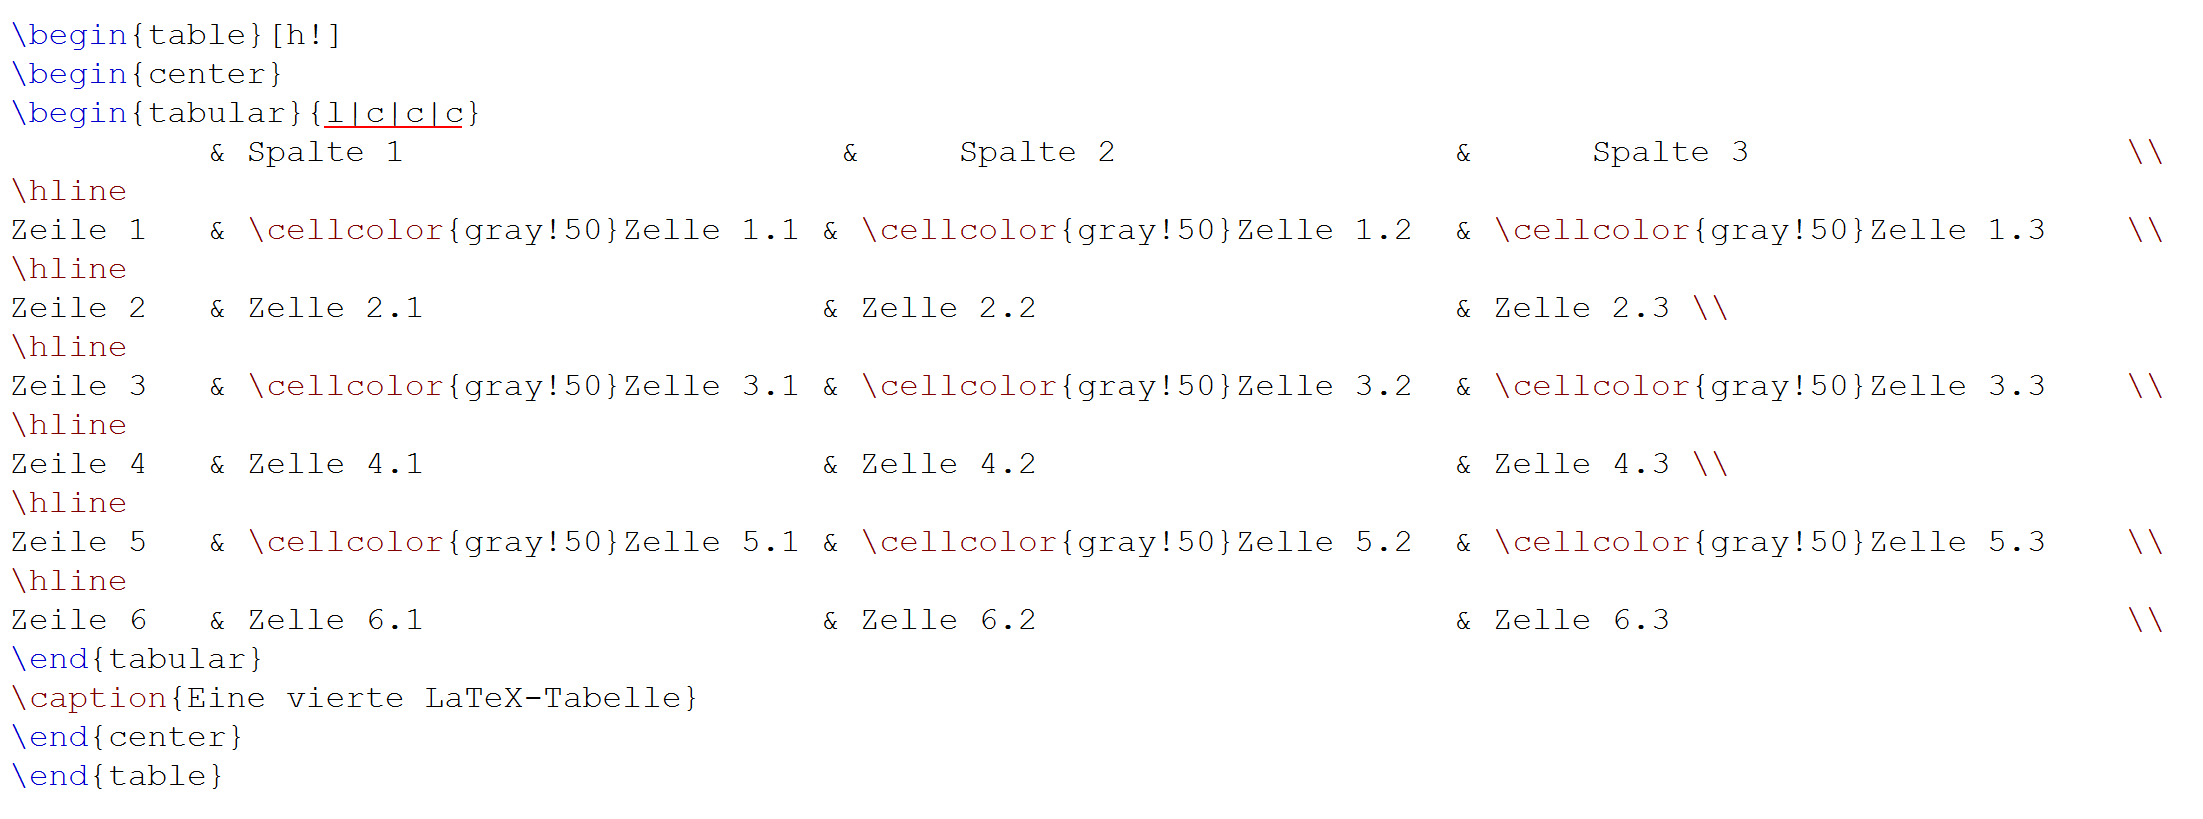
\includegraphics[width=0.75\textwidth]{./Bilder/Tabelle_4.png}}  
      \caption{Eine vierte LaTeX-Tabelle}
\end{figure} 

\newpage
Ein zweites Beispiel:


\begin{table}[h!]
\begin{center}
\begin{tabular}{p{1.5cm}|p{2.5cm}|p{2.5cm}|p{2.5cm}}
                   & \textbf{Spalte 1}              & \textbf{Spalte 2} & \textbf{Spalte 3}              \\
\hline
\textbf{Zeile 1}   & \cellcolor{gray!50}Zelle 1.1   & Zelle 1.2         & \cellcolor{gray!50}Zelle 1.3   \\
\hline
\textbf{Zeile 2}   & \cellcolor{gray!50}Zelle 2.1   & Zelle 2.2         & \cellcolor{gray!50}Zelle 2.3   \\
\hline
\textbf{Zeile 3}   & \cellcolor{gray!50}Zelle 3.1   & Zelle 3.2         & \cellcolor{gray!50}Zelle 3.3   \\
\hline
\textbf{Zeile 4}   & \cellcolor{gray!50}Zelle 4.1   & Zelle 4.2         & \cellcolor{gray!50}Zelle 4.3   \\
\hline
\textbf{Zeile 5}   & \cellcolor{gray!50}Zelle 5.1   & Zelle 5.2         & \cellcolor{gray!50}Zelle 5.3   \\
\hline
\textbf{Zeile 6}   & \cellcolor{gray!50}Zelle 6.1   & Zelle 6.2         & \cellcolor{gray!50}Zelle 6.3   \\
\end{tabular}
\caption{Eine fünfte LaTeX-Tabelle}
\end{center}
\end{table}



\begin{figure}[h!]
    \centering
      \fbox{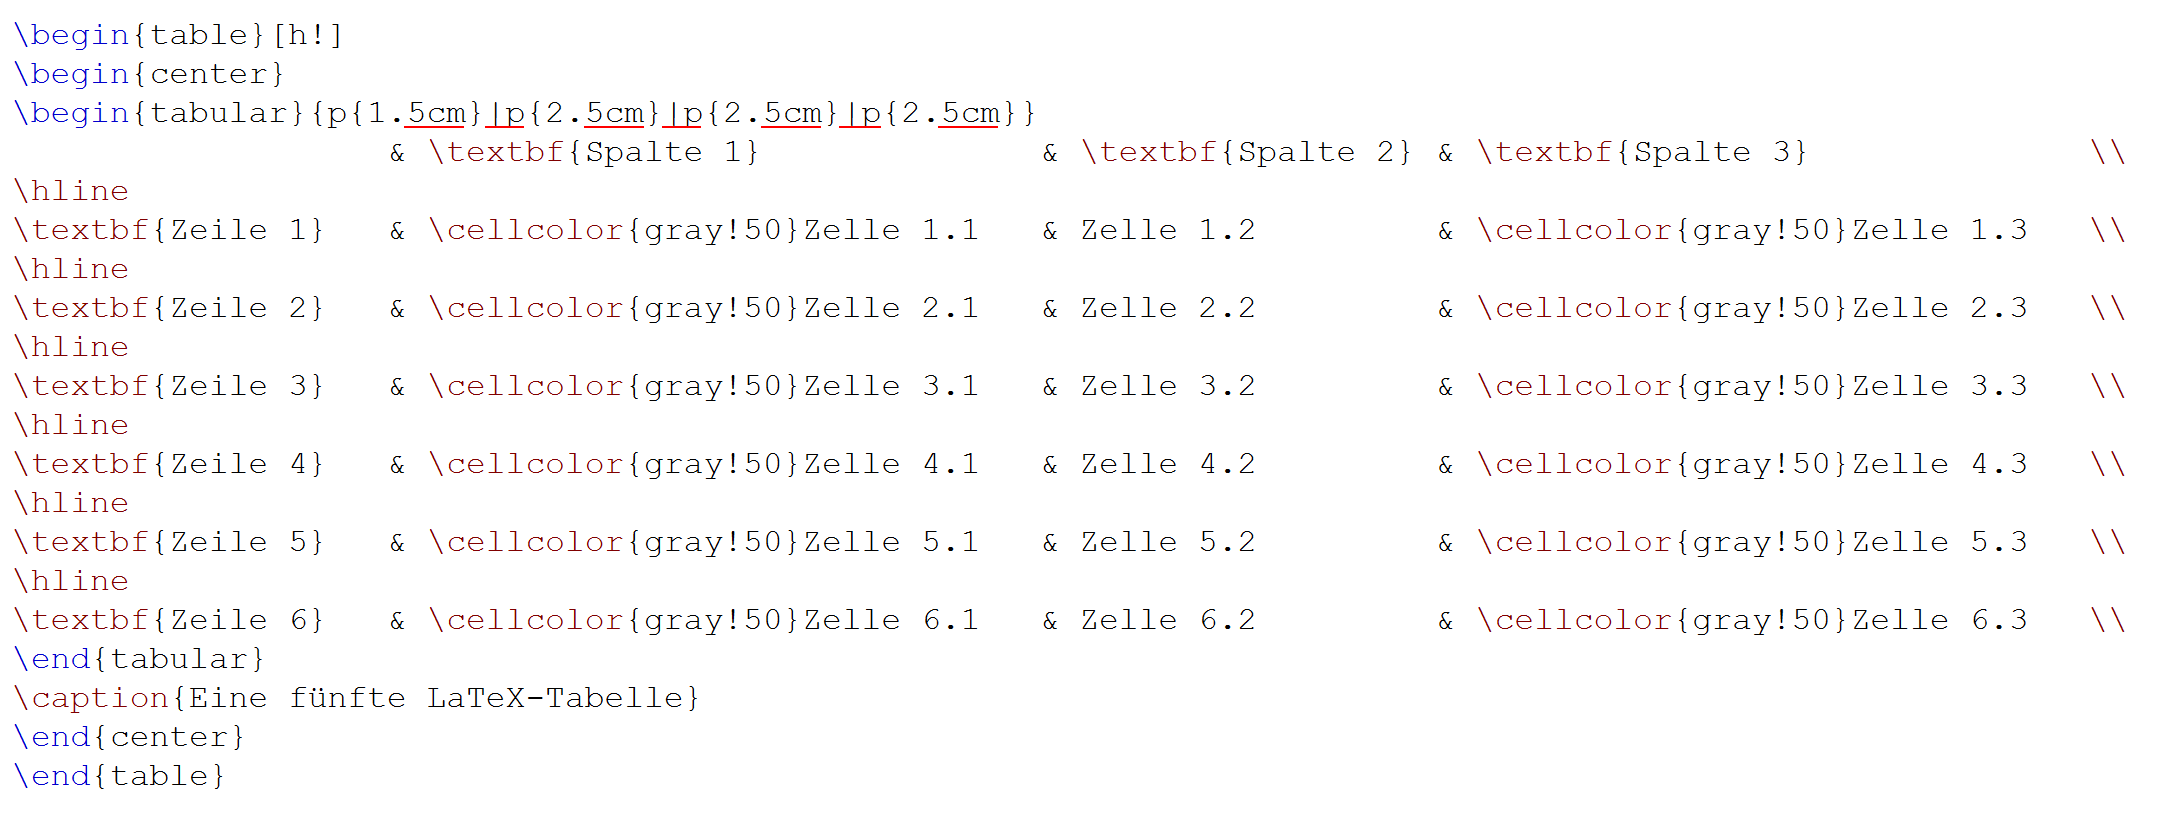
\includegraphics[width=0.7\textwidth]{./Bilder/Tabelle_5.png}}  
      \caption{Eine fünfte LaTeX-Tabelle}
\end{figure} 

Ein drittes Beispiel:


\begin{table}[h!]
\begin{center}
\begin{tabular}{c|c|c}
\rowcolor{gray!50} Spalte 1      &   Spalte 2     &   Spalte 3     \\
\hline
Zelle 1.1                        &   Zelle 1.2    &   Zelle 1.3    \\
\hline
Zelle 2.1                        &   Zelle 2.2    &   Zelle 2.3    \\
\end{tabular}
\caption{Eine sechste LaTeX-Tabelle}
\end{center}
\end{table}



\begin{figure}[h!]
    \centering
      \fbox{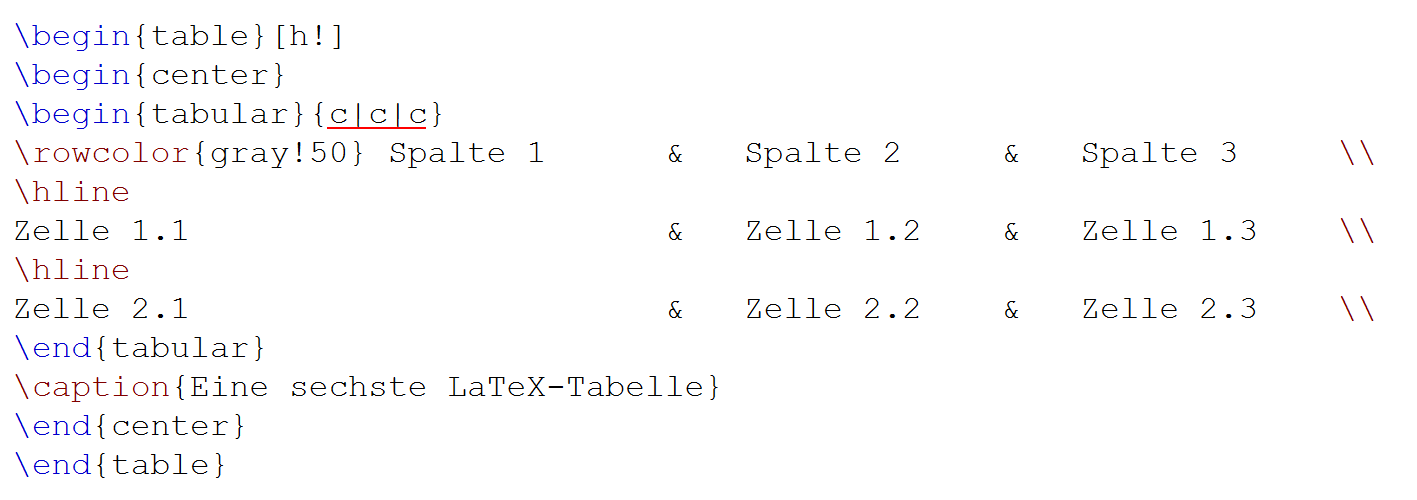
\includegraphics[width=0.7\textwidth]{./Bilder/Tabelle_6.png}}  
      \caption{Eine sechste LaTeX-Tabelle}
\end{figure} 

\textbf{Wichtig:} Die Formatierung der Tabellen in den \code{*.tex}-Dateien dient lediglich der Übersicht, resp. der Lesbarkeit des Codes für den Autor.
